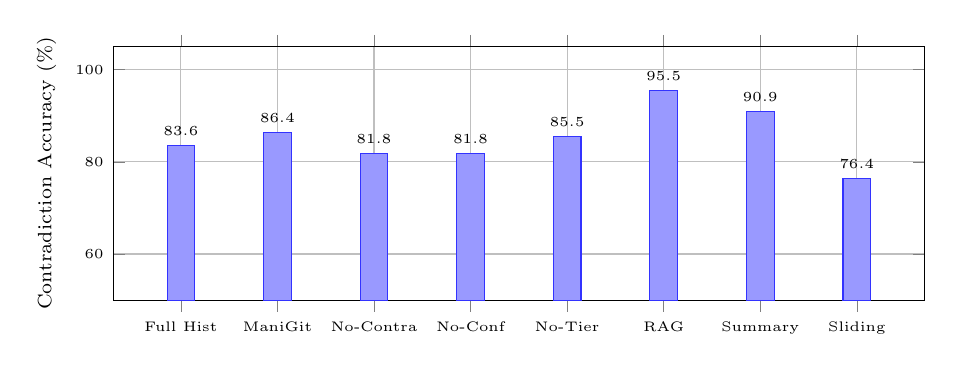
\begin{tikzpicture}
\begin{axis}[
    ybar,
    width=0.98\columnwidth, height=4.8cm,
    symbolic x coords={Full Hist, ManiGit, No-Contra, No-Conf, No-Tier, RAG, Summary, Sliding},
    xtick=data,
    ylabel={Contradiction Accuracy (\%)},
    ymin=50, ymax=105,
    nodes near coords,
    nodes near coords style={font=\tiny},
    grid=both,
    tick label style={font=\tiny},
    label style={font=\scriptsize}
]
\addplot[fill=blue!40, draw=blue!80] coordinates {
    (Full Hist, 83.6) (ManiGit, 86.4) (No-Contra, 81.8) (No-Conf, 81.8) (No-Tier, 85.5) (RAG, 95.5) (Summary, 90.9) (Sliding, 76.4)
};
\end{axis}
\end{tikzpicture}
